\chapter{Применение метода расчета траекторий движения индивидуальных жидких частичек} \label{ch:ch3}

\section{Введение} \label{sec:ch3/sec1}

В настоящей главе будет рассмотрено применение методики, представленной в предыдущей главе по отношению к более сложным случаям. В частности будут определены скорости дрейфа Стокса и траектории движения индивидуальных жидких частиц в случае, когда волновое возмущение свободной поверхности представляет из себя волновой пакет Стокса, а также будет рассмотрено влияние движущейся верхней среды и рассчитан дрейф и траектории движения жидких частиц в верхней движущейся среде; будет рассмотрено влияние поверхностного электрического заряда на переносные свойства волнового движения; и, наконец, будет рассмотрено совокупное влияние всех перечисленных факторов: будет произведен расчет скорости дрейфа Стокса и траекторий движения индивидуальных жидких частиц в двух контактирующих жидких средах, участвующих в относительном движении при условии, что на границе раздела распределен электрический заряд.

\section{Волновой пакет Стокса}\label{sec:WP}
\subsection{Введение}

В реальности крайне редко встречается распространение отдельной волны определенной длины, чаще формируются условия для возникновения цуга нескольких волн. Наиболее простой с точки зрения аналитического описания и экспериментальной реализации является волновой пакет Стокса. В настоящей главе обсуждается развитие методики, представленной ранее на случай распространения простейшего волнового пакета Стокса, состоящего из двух капиллярно~-- гравитационных волн одинаковой амплитуды  $ \zeta $ с волновыми числами  $ k_{\pm}=k \pm \Delta k $, отличающимися друг от друга на малую величину  $ 2 \Delta k \ll k $. Значение $ k $  характеризует волновое число несущей волны, а  $ \Delta k $~--- волновое число огибающей волнового пакета. Будет рассмотрено влияние различных дестабилизирующих факторов на скорость массопереноса и на характер движения индивидуальных жидких частиц, таких как поверхностный электрический заряд и тангенциальный разрыв скоростей на границе раздела двух жидких сред.

\subsection{Математическая формулировка задачи}

Пусть в декартовой системе координат $ Oxyz $, в которой ось $ Oz $  направлена вертикально вверх против направления действия поля сил тяжести $ \mathbf{g} $  расположен слой идеальной несжимаемой жидкости, занимающий область пространства  $ -\infty <z<\xi $. А по его свободной поверхности $ z=\xi $  распространяется простейший волновой пакет Стокса, состоящий из двух капиллярно~-- гравитационных волн с одинаковой амплитудой $ \zeta $  и волновыми числами $ k_{\pm} $. Направление распространения совпадает с положительным направлением оси  $ Ox $. В простейшем случае можно считать, что движение жидкости не зависит от горизонтальной координаты  $ y $. Будем решать задачу в приближении волн малой амплитуды. Тогда уравнения движения представляют из себя известные уравнения гидродинамики \parencite{Landau}:
\begin{align}
\begin{aligned}
z<\xi: \mspace{108mu} \partial_{t} \mathbf{U}+\left( \mathbf{U} \cdot  \nabla \right) \mathbf{U} &= - \dfrac{\nabla p}{\rho}+\mathbf{g} ; \mspace{108mu}
\\
 \nabla \cdot \mathbf{U}&=0;\label{EulerPack}
\end{aligned}
\end{align}
с граничными условиями на верхней границе:
\begin{align}
\begin{aligned}
z=\xi: \mspace{160mu} \partial_{t} \xi-v &= - u \partial_{x}\xi ;\mspace{160mu}
\\
 p=-\gamma \partial_{xx}&\xi \left( 1+\left( \partial_{x}\xi \right)^{2}\right)^{-3/2} ;\label{GUPack}
\end{aligned}
\end{align}
и с условием затухания движения на бесконечности:
\begin{equation}
z \rightarrow -\infty: \mspace{108mu} u=0; \mspace{108mu} v=0. \mspace{108mu}
\end{equation}

Здесь $ \mathbf{U}\left( x, z, t \right) = \nabla \varphi = u \left( x, z, t\right) \mathbf{e}_{x}+v \left( x, z, t\right) \mathbf{e}_{z} $~--- поле скоростей в обозначениях Эйлера, $ \varphi $~--- гидродинамический потенциал,  $ t $~--- время, $ p $~--- давление, а $ \gamma $~--- поверхностное натяжение жидкости. Для определения скорости дрейфа воспользуемся описанной выше процедурой решения: используем метод разложения по малому параметру, снос граничных условий на равновесную поверхность $ z=0 $  и разбиение задачи на порядки малости до второго порядка малости включительно. Представим неизвестные функции в виде разложения в ряд по малому параметру, пропорциональному амплитуде волнового движения   $ \varepsilon = \zeta k $:
\begin{equation*}
\begin{pmatrix}
\xi
\\
\varphi
\end{pmatrix}= \varepsilon \begin{pmatrix}
\xi_{1}
\\
\varphi_{1}\end{pmatrix}+ \varepsilon^{2} \begin{pmatrix}
\xi_{1}
\\
\varphi_{1}\end{pmatrix}+ O\left( \varepsilon^{3}\right)
\end{equation*}
	  	
Произведем линеаризацию граничных условий~\eqref{GUPack} по методике, описанной в предыдущей главе. Распишем математическую формулировку задачи в первом и во втором по амплитуде волны порядке малости. Задача первого порядка малости записывается в виде:
\begin{align}
&z<0 : \mspace{192mu} \Delta \varphi_{1}=0; \label{EulPack1} \mspace{192mu}
\\
&z=0 : \mspace{172mu} \partial_{t}\xi_{1} -\partial_{z} \varphi_{1}=0 ; \label{GUPack1}
\\
& \mspace{180mu}  \rho g \xi_{1}-\rho \partial_{t} \varphi_{1}+\gamma \partial_{xx}\xi_{1}=0 ; \label{GUPack2}
\\
& z\rightarrow -\infty :\mspace{165mu}\nabla \varphi_{1} \rightarrow 0.\label{BeskPack1}
\end{align}

Задача второго порядка малости запишется следующим образом: 
\begin{align}
&z<0 : \mspace{192mu} \Delta \varphi_{2}=0; \label{EulPack2} \mspace{192mu}
\\
&z=0 : \mspace{108mu} \partial_{t}\xi_{2} -\partial_{z} \varphi_{2}=\xi_{1} \partial_{zz}\varphi_{1} - \partial_{x} \varphi_{1} \partial_{x} \xi{1} ; 
\\
& \qquad  \rho g \xi_{2}-\rho \partial_{t} \varphi_{2}+\gamma \partial_{xx}\xi_{2}=\rho \xi_{1} \partial_{zt} \varphi_{1} + \dfrac{\rho}{2} \left(\partial_{x} \varphi_{1} \right)^{2}+ \dfrac{\rho}{2} \left(\partial_{z} \varphi_{1} \right)^{2} ;
\\
& z\rightarrow -\infty :\mspace{165mu} \nabla \varphi_{2} \rightarrow 0.\label{BeskPack2}
\end{align}

\subsection{Решение задачи}

Решение задачи~\eqref{EulPack1}~---~\eqref{BeskPack1}  в виде совокупности бегущих волн легко находится стандартными методами математической физики и имеет вид:
\begin{equation}
\xi_{1}=\zeta \cos \left( \omega_{+} t - k_{+} x \right) + \zeta \cos \left( \omega_{-} t - k_{-} x \right);
\label{ReshXiPack}
\end{equation}
\begin{equation}
\varphi_{1}=-\zeta \dfrac{\omega_{+}}{k_{+}}\exp \left( k_{+} z\right) \sin \left( \omega_{+} t- k_{+} x \right) -\zeta \dfrac{\omega_{-}}{k_{-}}\exp \left( k_{-} z\right) \sin \left( \omega_{-} t- k_{-} x \right); 
\label{ReshPhiPack}
\end{equation}
	 
Здесь $ \omega_{\pm} $~--- частоты волнового движения, волн, составляющих пакет. Они связаны с волновыми числами соответствующих волн несложным образом, определяемым из дисперсионного уравнения:
\begin{equation}
\omega_{\pm}=\omega \pm \Delta \omega = \sqrt{g k _{\pm} \left( 1+ k_{\pm}^{2} \alpha^{2} \right)}
\label{DispUrPack}
\end{equation}
	  	
Здесь стоит отметить, что в дисперсионное уравнение~\eqref{DispUrPack} неявным образом (в составе волновых чисел $ k_{\pm} $ ) входит параметр $ \Delta k $, считающийся малым, а символ $ \alpha= \sqrt{\gamma/\rho g} $  обозначает капиллярную постоянную жидкости. 

Выражение для отклонения границы раздела $ \xi_{1} $ от равновесного положения~\eqref{ReshXiPack} при помощи тригонометрических преобразований легко сводится к виду \parencite{Ostrovsky}:
\begin{equation}
\xi_{1}=2\zeta \cos \left( \omega t - k x \right) \cos \left( \Delta \omega t - \Delta k x \right)
\label{WavePacket}  
\end{equation}
	  	
Из соотношения~\eqref{WavePacket} естественным образом выделяется два временных масштаба $ T=2\pi/\omega $~--- период несущей волнового пакета, характеризующий быстрые изменения во времени и $ \tau=2\pi/\Delta \omega $~--- период огибающей, характеризующий медленно меняющиеся процессы. 
Задача второго порядка малости~\eqref{EulPack2}~---~\eqref{BeskPack2}  представляет из себя однородное уравнение с неоднородными граничными условиями на верхней границе. Явный вид неоднородностей получим, подставив найденное решение задачи первого порядка малости~---  в~правые части граничных условий~\eqref{GUPack1}~---~\eqref{GUPack2}.
 
Как и в предыдущих разобранных случаях в неоднородностях есть составляющие, быстро меняющиеся со временем. Эти слагаемые отвечают за циклические движения жидких частичек и не представляют интереса для нашего рассмотрения, поскольку в круговых движениях жидких частиц лидирующими являются слагаемые первого порядка малости по амплитуде волнового движения. В предыдущих случаях неоднородность представляла из себя только такие слагаемые, и поэтому на этом этапе заканчивалось решение задачи второго порядка малости и дрейфовая скорость определялась только интегральными слагаемыми в формуле~\eqref{Pereh}. Однако в случае распространения волнового пакета расчет первого слагаемого в правой части  не столь тривиален. Дело в том, что во втором порядке малости возникают дополнительные добавки к Эйлеровой скорости, которые медленно меняются со временем (по сравнению с периодом волнового движения) и отвечают за медленно изменяющееся дрейфовое течение. Ограничимся определением только таких составляющих скорости второго порядка малости в переменных Эйлера. В явном виде правые части граничных условий  выглядят следующим образом:
\begin{equation}
\xi_{1}\partial_{zz}\varphi_{1}-\partial_{x}\varphi_{1}\partial_{x}\xi_{1}=-2\zeta^{2}\Delta k \omega \sin \left( 2 t \Delta \omega - 2 x \Delta k \right) + \Pi \left( t \right);
\label{Neodn1}
\end{equation}
\begin{multline}
\rho \xi_{1} \partial_{zt} \varphi_{1}+\dfrac{\rho}{2}\left( \partial_{x}\varphi_{1}\right)^{2}+\dfrac{\rho}{2}\left( \partial_{z}\varphi_{1}\right)^{2}=\\=-2\zeta^{2}\rho \Delta \omega^{2} \cos \left( 2 t \Delta \omega - 2 x \Delta k \right) + \Pi \left( t \right).
\label{Neodn2}
\end{multline}

Здесь для краткости записи принято, что слагаемые $ \Pi \left( t \right) $  представляют из себя совокупность функций синуса и косинуса, в аргументе которых содержится произведение  $ \omega t $ и которые, соответственно, быстро меняются со временем, отвечая за циклические движения жидких частичек.

Из вида неоднородностей~\eqref{Neodn1}~---~\eqref{Neodn2} следует, что решение задачи~\eqref{EulPack2}~---~\eqref{BeskPack2} следует искать в виде бегущей волны с аргументом  $ \theta\perm= 2 t \Delta \omega \perm- 2 x \Delta k $. А зависимость от вертикальной координаты $ z $  ищется такой, чтобы удовлетворять уравнению Лапласа и условию прекращения движения на дне. Такое решение несложно найти. Приведем только горизонтальную составляющую скорости, поскольку для вычисления горизонтальной скорости дрейфа по формуле  другие переменные нам не понадобятся:
\begin{equation*}
u_{2}=2\zeta^{2}\omega \Delta k \cos \left( 2 t V_{g} \Delta k - 2 x \Delta k \right) \exp \left( 2 z \Delta k \right)
\end{equation*}
Здесь надо понимать, что приведена только интересующая нас часть решения задачи второго порядка малости, в нашем рассмотрении нет необходимости решать задачу второго порядка малости целиком. Также стоит пояснить смысл произведенной замены  $ \Delta \omega \rightarrow V_{g} \Delta k $. В дисперсионное уравнение входит небольшая добавка к волновому числу  $ \Delta k $, считая ее малой и разлагая частоту волнового движения в ряд Маклорена, в линейном приближении получим:
\begin{equation*}
\omega_{\pm}=\omega \pm \Delta \omega = \omega \pm \partial_{k} \omega \Delta k.
\end{equation*}

Причем частная производная  $ \partial_{k}\omega = V_{g} $ играет роль групповой скорости волнового пакета. Для нашего рассмотрения неинтересно производить расчет вертикальной составляющей в связи с отсутствием движения всей жидкости как целого в вертикальных направлениях. 

Выпишем в явном виде компоненты лагранжевой скорости индивидуальной жидкой частички с точностью до слагаемых первого порядка малости. В~линейном приближении скорость в описании Эйлера и в описании Лагранжа формально совпадают \parencite{Landau}, но при этом координаты, входящие в уравнения, меняют свой смысл на лагранжевы координаты (в нашем рассмотрении это начальные координаты жидкой частицы):
\begin{gather}
\begin{gathered}
u_{L1}=\zeta \omega_{-}\exp \left( k_{-} z_{0}\right) \cos \left( \omega_{-} t - k_{-} x_{0} \right)+\\
+\zeta \omega_{+}\exp \left( k_{+} z_{0}\right) \cos \left( \omega_{+} t - k_{+} x_{0} \right)
\label{ul1Pack}
\end{gathered}
\\
\begin{gathered}
v_{L1}=-\zeta \omega_{-}\exp \left( k_{-} z_{0}\right) \sin \left( \omega_{-} t - k_{-} x_{0} \right)-\\
-\zeta \omega_{+}\exp \left( k_{+} z_{0}\right) \sin \left( \omega_{+} t - k_{+} x_{0} \right)
\label{vl1Pack}
\end{gathered}
\end{gather}
	  	
Далее, следуя методу определения лагранжевой скорости, необходимо произвести вычисление интегральных слагаемых в формуле~\eqref{Pereh}. Заинтересованный читатель легко произведет эти вычисления при помощи любого математического пакета программ. Чтобы избежать загромождение изложения, приведем уже готовое выражение для горизонтальной составляющей лагранжевой скорости:
\begin{equation*}
u_{L}=D+\Pi,
\end{equation*}
где $ \Pi $~--- быстроменяющиеся (по сравнению с периодом огибающей волнового пакета) слагаемые, отвечающие  за колебательные движения жидкой частички около некоторого среднего положения, а символом $ D $  обозначены слагаемые, соответствующие медленному дрейфовому движению этого среднего положения. В явном виде дрейфовая скорость выглядит следующим образом:
\begin{gather}
\begin{gathered}
D=\zeta^{2} \left[ \left( k \omega +\Delta k \left( k V_{g}+\omega \right) \right) \exp \left( 2 k_{+}z \right) + \right.\\
+\left( k \omega - \Delta k \left( k V_{g}+\omega \right) \right) \exp \left( 2 k_{-}z \right)+\\
+2 k \omega \cos \left( 2 t V_{g} \Delta k - 2 x \Delta k \right) \exp \left( 2 k z \right) +\\
\left. +2 \omega \Delta k \cos \left( 2 t V_{g} \Delta k - 2 x \Delta k \right) \exp \left( 2 \Delta k z \right) \right]
\label{DriftPack}
\end{gathered}
\end{gather}
	  	
Важно отметить, что расчет дрейфовой скорости  произведен в линейном приближении по отклонению волновых чисел волн в пакете друг от друга  $ \Delta k $. Слагаемые, пропорциональные $ \Delta k $  в более высоких степенях отбрасывались в силу малости и громоздкости. Такое приближение должно удовлетворить большинство расчетных задач, однако при помощи представленной методики можно воспроизвести дрейфовую скорость целиком . Полная дрейфовая скорость не приведена здесь в силу неинформативности отброшенных слагаемых. 

Сравним скорость дрейфового движения~\eqref{DriftPack} со скоростью классического дрейфа Стокса~\eqref{DriftStokes}. Первое отличие, бросающееся в глаза~--- зависимость скорости дрейфа  от времени, которое должно наблюдаться на небольших интервалах времени в эксперименте (время наблюдения $ t_{obs} $  должно быть сравнимо с периодом несущей волнового пакета $ T $ ). Если же время наблюдения велико (по сравнению с периодом огибающей волнового пакета $ t_{obs}\gg T $ ), то имеет смысл говорить об усредненной скорости дрейфового движения за период огибающей волнового пакета  $ \left\langle D \right\rangle   $:
\begin{gather}
\begin{gathered}
 \left\langle D\right\rangle  = \zeta^{2}\left[ \left( k \omega + \Delta k \left( k V_{g} + \omega \right) \right) \exp \left( 2 k_{+} z \right) + \right. \\
 \left. + \left( k \omega - \Delta k \left( k V_{g} + \omega \right) \right) \exp \left( 2 k_{-} z \right) \right]
 \label{SRDrift}
 \end{gathered}
\end{gather}
	  	
На рисунке~\ref{fig:Drift} изображены скорости классического дрейфа Стокса~\eqref{DriftStokes}, а также скорости дрейфа, определяемые соотношениями~\eqref{DriftPack} и~\eqref{SRDrift} в безразмерных переменных $ \rho=g=\gamma=1 $для жидкости с параметрами воды и параметрами волнового движения $ k=k_{cr} $, $ \Delta k= 0.01 k_{cr} $, $ \zeta=0.05 \lambda_{cr} $.
\begin{figure}[h]
\centering
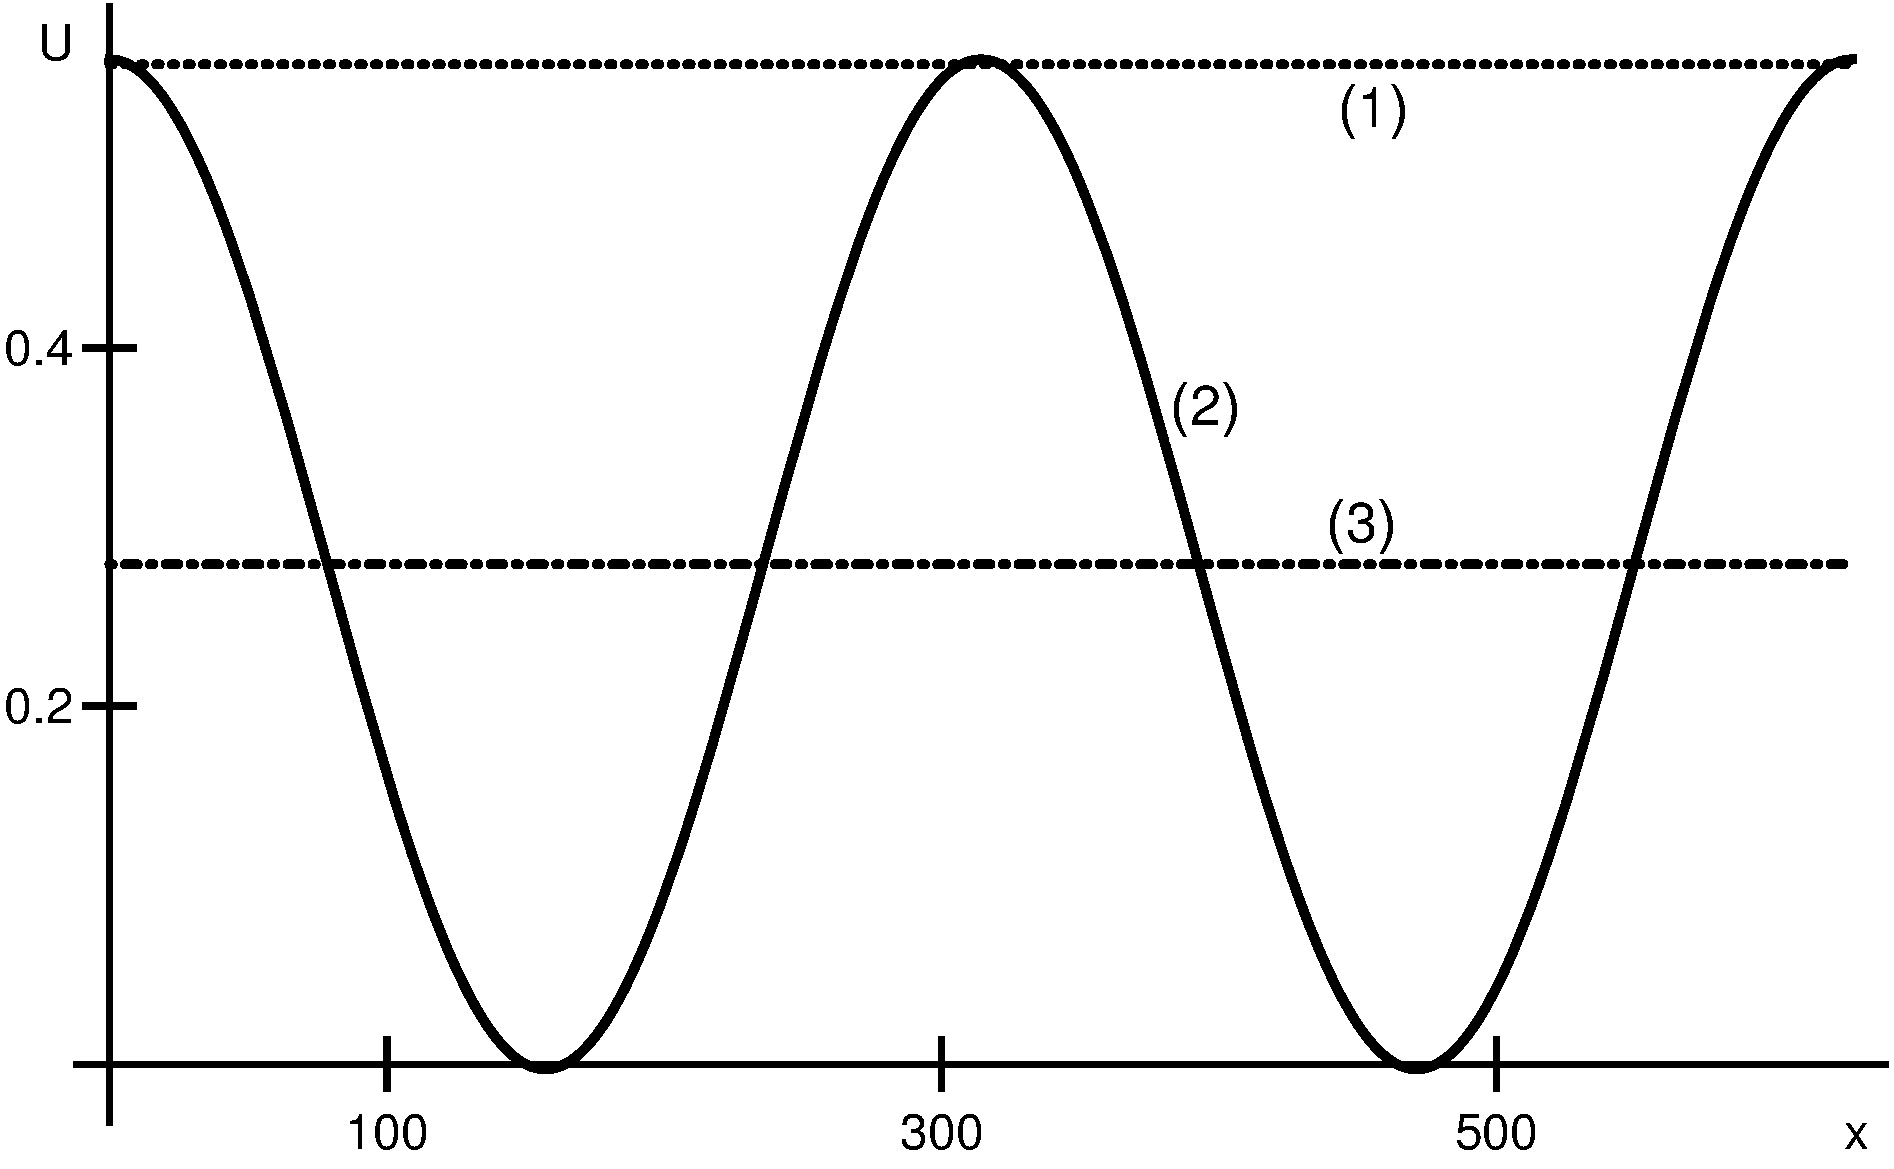
\includegraphics[scale=0.5]{Drift_Packet.pdf}
\caption{Скорость классического дрейфа Стокса (кривая 1), дрейфа Стокса, инициированного волновым пакетом Стокса (кривая 2) и среднего значения дрейфа Стокса, инициированного волновым пакетом Стокса (кривая~3)}\label{fig:Drift}
\end{figure}
Периодическое изменение скорости дрейфа связано с тем, что скорость дрейфа пропорциональна амплитуде волнового движения, а в случае, когда возмущение свободной поверхности представляет из себя волновой пакет Стокса амплитуда модулирована. Именно эта модуляция и вызывает временную зависимость скорости дрейфа. Расчеты показывают, что усредненная за период огибающей волнового пакета скорость дрейфа  принимает значения примерно в два раза меньшие, чем скорость классического дрейфа Стокса. Такая же тенденция должна сохраняться для произвольного цуга волн. Таким образом в эксперименте дрейф Стокса нужно ожидать в разы меньшим, чем это предсказывает классическая теория Стокса.

Произведем поправку лагранжевой скорости жидкой частички~\eqref{ul1Pack}~---~\eqref{vl1Pack} на скорость дрейфового движения в соответствии с разработанной методикой. С учетом этой поправки усовершенствованный вид лагранжевых компонент скорости жидкой частицы с точностью до лидирующих слагаемых запишется следующим образом:
\begin{gather}
\begin{gathered}
u_{L}\left( x_{0}, z_{0}, t \right)=\zeta \omega_{-}\exp \left( k_{-} z_{0}\right) \cos \left( \left( \omega_{-}-k_{-} D\right) t - k_{-} x_{0} \right)+\\
+\zeta \omega_{+}\exp \left( k_{+} z_{0}\right) \cos \left( \left( \omega_{+}-k_{+} D\right)  t - k_{+} x_{0} \right)+D
\label{ulPackTrue}
\end{gathered}	  
\end{gather}
\begin{gather}	
\begin{gathered}
v_{L}\left( x_{0}, z_{0}, t \right)=-\zeta \omega_{-}\exp \left( k_{-} z_{0}\right) \sin \left( \left( \omega_{-}-k_{-} D\right) t - k_{-} x_{0} \right)-\\
-\zeta \omega_{+}\exp \left( k_{+} z_{0}\right) \sin \left( \left( \omega_{+}-k_{+} D\right)  t - k_{+} x_{0} \right)
\label{vlPackTrue}
\end{gathered}
\end{gather}	  	
	  	
Прямое интегрирование выражений~\eqref{ulPackTrue}~---~\eqref{vlPackTrue}  позволяет получить выражения для параметрической формы записи траекторий движения индивидуальных жидких частиц.
\begin{equation}
X=x_{0}+\int_{0}^{t}u_{L}\left( x_{0}, z_{0}, \tau \right)d\tau
\label{XPack}
\end{equation}
\begin{equation}
Z=z_{0}+\int_{0}^{t}v_{L}\left( x_{0}, z_{0}, \tau \right)d\tau
\label{ZPack}
\end{equation}	  	
	  	
В явном аналитическом виде не удается получить простые выражения, удобные для анализа. При необходимости выражения для траекторий движения индивидуальных жидких частиц можно получить, высчитывая интегралы~\eqref{XPack}~---~\eqref{ZPack} численно.

Однако, несмотря на отсутствие выражений для траекторий в явном виде можно сделать некоторые выводы о характере движения. Можно заметить, что частота кругового движения индивидуальной жидкой частички окажется меньше, чем частота волновой моды, инициировавшей это движение. Это связано с необходимостью согласования движения индивидуальных жидких частиц и волнового движения свободной поверхности.

\subsection{Результаты}

В случае инициации дрейфового движения волновым пакетом Стокса результаты наблюдения за скоростью дрейфа существенно будут зависеть от времени наблюдения. На малых временах наблюдения (сравнимых с периодом несущей волнового пакета и много меньших периода огибающей) будет наблюдаться зависимость скорости дрейфа~\eqref{DriftPack} от времени и ее периодический характер. На временах, заметно превышающих период огибающей волнового пакета, имеет смысл говорить об усредненной скорости дрейфового движения~\eqref{SRDrift}. Ее величина для простейшего волнового пакета Стокса оказывается примерно вдвое меньшей, чем скорость классического дрейфа Стокса. По-видимому, подобная тенденция сохранятся и для произвольного волнового пакета: в эксперименте стоит ожидать скорость дрейфа в разы меньшую, чем это предсказывает классическая теория.

\section{Влияние тангенциального разрыва скоростей на скорости индивидуальных жидких частиц и скорости дрейфа Стокса, вызванного распространением волнового пакета Стокса по границе раздела жидких сред}
  
В настоящем разделе рассмотрено совокупное действие факторов, отдельное действие которых обсуждалось в предыдущей главе и в предыдущем разделе. Рассчитывается дрейф и траектории движения индивидуальных жидких частиц в двух контактирующих жидких средах в зависимости от скорости относительного движения этих сред также, как и в главе \ref{ch:ch2}. При этом граница раздела считается возмущенной простейшим волновым пакетом Стокса, как в предыдущем разделе \ref{sec:WP}.

Математическая формулировка задачи формально совпадает с выражениями~\eqref{Euler}~---~\eqref{BeskUsl}. Используя разложение по малому параметру и производя снос граничных условий с возмущенной поверхности на уровень равновесной границы раздела  $ z=0 $ получим задачи первого и второго порядка малости по амплитуде волнового движения. Их математическая запись окажется аналогичной ~\eqref{Eul1}~---~\eqref{Besk1} и~\eqref{Eul2}~---~\eqref{Besk2} соответственно. Решение задачи первого порядка малости в виде совокупности двух бегущих волн находится стандартными методами математической физики и выглядит следующим образом:
\begin{gather}
\xi_{1}=\zeta \cos \left( \omega_{+} t -k_{+} x \right)+\zeta \cos \left( \omega_{-} t -k_{-} x \right)\label{ReshPackKH1Xi}
\\
\begin{gathered}
\varphi_{1} = -\zeta \exp \left( k_{+} z\right) \dfrac{\omega_{+}}{k_{+}}\sin \left( \omega_{+} t -k_{+} x \right)-
\\
 -\zeta \exp \left( k_{-} z\right) \dfrac{\omega_{-}}{k_{-}}\sin \left( \omega_{-} t -k_{-} x \right)\label{ReshPackKH1Phi}
 \end{gathered}
\\
\begin{gathered}
\varphi'_{1} = -\zeta \exp \left(- k_{+} z\right) \dfrac{k_{+} U_{0}-\omega_{+}}{k_{+}}\sin \left( \omega_{+} t -k_{+} x \right) -\\
-\zeta \exp \left( k_{-} z\right) \dfrac{k_{-}U_{0}-\omega_{-}}{k_{-}}\sin \left( \omega_{-} t -k_{-} x \right)
\label{ReshPackKH1Phi'}
\end{gathered}
\end{gather}

	  	
Здесь в качестве $ \omega_{\pm}=\omega \pm \Delta \omega =\omega \pm \partial_{k} \omega \Delta k $  как и в предыдущем пункте приняты циклические частоты волновых движений, составляющих пакет Стокса. Однако дисперсионное уравнение, обеспечивающее связь между частотой и волновым числом совпадает с дисперсионным уравнением~\eqref{DispUrKH}. 

В этой задаче аналогично задаче из предыдущего пункта \ref{sec:WP} возникают естественные временные масштабы: быстрый $ T=2\pi/\omega $  и медленный  $ \tau = 2\pi/\Delta \omega $. Подставляя решение~\eqref{ReshPackKH1Xi}~---~\eqref{ReshPackKH1Phi'} в правые части граничных условий ~\eqref{GU2},  получим граничные условия задачи второго порядка малости по амплитуде волны в явном виде. При этом слагаемые, быстроменяющиеся со временем и не оказывающие влияния на скорость дрейфового движения обозначим  $ \Pi \left( t \right) $:
\begin{gather}
\begin{gathered}
\partial_{t}\xi_{2}-\partial_{z}\varphi_{2}=-2\zeta^{2}\Delta k \omega \sin \left( 2 \Delta \omega - 2 \Delta k x \right) +\zeta^{2} \Pi \left( t \right)\\
\partial_{t}\xi_{2}+U_{0}\partial_{x}\xi_{2}-\partial_{z}\varphi'_{2}=\\
=2 \zeta^{2} \left( U_{0}^{2}\Delta k^{2}\rho'-2U_{0}\Delta k \Delta \omega \rho' +\Delta \omega^{2} \rho' - \Delta \omega^{2} \rho \right) \times\\
\times \cos \left( 2 \Delta \omega t - 2 \Delta k x \right) + \zeta^{2} \Pi \left( t \right)\\
g \xi_{2} \left( \rho' - \rho \right) - \rho \partial_{t} \varphi_{2} + \rho' \partial_{t} \varphi'_{2} + \rho' U_{0} \partial_{x} \varphi'_{2}+\gamma \partial_{xx}\xi_{2}=\\
=2 \zeta^{2} \left( k U_{0}\Delta k - \Delta k \omega \right) \sin \left( 2 \Delta \omega t - 2 \Delta k x \right) + \zeta^{2} \Pi \left( t \right)
\label{RPPacketKH}
\end{gathered}
\end{gather}
	  		  	
Как и в предыдущих пунктах для рассмотрения настоящей задачи нет необходимости решать задачу второго порядка малости полностью. Поскольку быстроменяющиеся со временем слагаемые не вносят вклада в дрейфовые движения, а лидирующими слагаемыми в круговом движении являются слагаемые первого порядка малости, достаточно решить «усеченную» задачу второго порядка малости с отброшенными слагаемыми вида  $ \Pi \left(t \right) $. Соответствующее решение для компонент поля скоростей в нижней $ u_{d} $  и в верхней $ u'_{d} $  жидкостях имеют вид:
\begin{equation}
u_{d}=-2\zeta^{2}\Delta k \omega e^{2 z \Delta k} \cos \left( 2 \Delta \omega t-2 \Delta k x \right)
\label{udPacketKH}
\end{equation}
\begin{equation}
u'_{d}=2\zeta^{2}\Delta k\left( k U_{0}- \omega \right) e^{-2 z \Delta k} \cos \left( 2 \Delta \omega t-2 \Delta k x \right)
\label{ud'PacketKH}
\end{equation}
	  		  	
Соотношения~\eqref{ReshPackKH1Phi}~---~\eqref{ReshPackKH1Phi'},~\eqref{udPacketKH}~---~\eqref{ud'PacketKH}  представляют части эйлеровой компоненты скорости течения, через которые вычисляется лагранжевая скорость жидкой частицы с точностью до лидирующих слагаемых (первого порядка малости для кругового и второго порядка малости для дрейфового движения). Подставляя~\eqref{ReshPackKH1Phi}~---~\eqref{ReshPackKH1Phi'},~\eqref{udPacketKH}~---~\eqref{ud'PacketKH} в~\eqref{Pereh} и выделяя медленно меняющиеся слагаемые аналогично тому, как это делалось в разделе~\ref{sec:WP} получим выражения для скорости дрейфа в нижней $ U_{drift} $  и в верхней среде  $ U'_{drift} $:
\begin{gather}
\begin{gathered}
U_{drift}=\zeta^{2}e^{2k_{+}z}\left( k \omega +\Delta k \omega +k \Delta \omega \right) +\zeta^{2}e^{2k_{-}z}\left( k \omega -\Delta k \omega -k \Delta \omega \right)+\\
+ 2 \zeta^{2} k \omega e^{2 k z} \cos \left( 2 \Delta \omega t - 2 \Delta k x \right) + u_{d}\\
U'_{drift}=\zeta^{2}e^{-2k_{+}z}\left( k \Omega +\Delta k \Omega +k \Delta \omega \right) +\zeta^{2}e^{-2k_{-}z}\left( k \Omega -\Delta k \Omega -k \Delta \omega \right)+\\
+ 2 \zeta^{2} k \Omega e^{-2 k z} \cos \left( 2 \Delta \omega t - 2 \Delta k x \right) + u'_{d}+U_{0}
\label{UdriftPack}
\end{gathered}
\end{gather}
	  		  	
Используя описанную методику запишем скорость индивидуальной жидкой частички в описании Лагранжа с точностью до лидирующих слагаемых каждого типа движения в нижней жидкости:	\begin{gather}
\begin{gathered}
u_{L}\left( x_{0}, z_{0}, t \right)=\zeta \omega_{-}\exp \left( k_{-} z_{0}\right) \cos \left( \left( \omega_{-}-k_{-} U_{drift}\right) t - k_{-} x_{0} \right)+\\
+\zeta \omega_{+}\exp \left( k_{+} z_{0}\right) \cos \left( \left( \omega_{+}-k_{+} U_{drift}\right)  t - k_{+} x_{0} \right)+U_{drift}\\
v_{L}\left( x_{0}, z_{0}, t \right)=-\zeta \omega_{-}\exp \left( k_{-} z_{0}\right) \sin \left( \left( \omega_{-}-k_{-} U_{drift}\right) t - k_{-} x_{0} \right)-\\
-\zeta \omega_{+}\exp \left( k_{+} z_{0}\right) \sin \left( \left( \omega_{+}-k_{+} U_{drift}\right)  t - k_{+} x_{0} \right)
\label{ULPackKH}
\end{gathered}
\end{gather}	  	
	  	
В верхней жидкости лагранжевая скорость жидких частичек выглядит следующим образом:
\begin{gather}
\begin{gathered}
u'_{L}\left( x_{0}, z_{0}, t \right)=U_{drift}+\zeta \left(k_{-}U_{0}- \omega_{-}\right)\exp \left( k_{-} z_{0}\right) \times \\
\times \cos \left( \left( \omega_{-}-k_{-} U'_{drift}\right) t - k_{-} x_{0} \right)+\\
+\zeta \left(k_{+}U_{0}- \omega_{+}\right)\exp \left( k_{+} z_{0}\right) \cos \left( \left( \omega_{+}-k_{+} U'_{drift}\right)  t - k_{+} x_{0} \right)\\
v'_{L}\left( x_{0}, z_{0}, t \right)=-\zeta \left(k_{-}U_{0}- \omega_{-}\right)\exp \left( k_{-} z_{0}\right) \times\\
\times \sin \left( \left( \omega_{-}-k_{-} U'_{drift}\right) t - k_{-} x_{0} \right)-\\
-\zeta \left(k_{+}U_{0}- \omega_{+}\right)\exp \left( k_{+} z_{0}\right) \sin \left( \left( \omega_{+}-k_{+} U'_{drift}\right)  t - k_{+} x_{0} \right)
\label{UL'PackKH}
\end{gathered}
\end{gather}	  
	  	
Интегрирование выражений~\eqref{ULPackKH}~---~\eqref{UL'PackKH} по времени позволит получить выражения для траекторий движения индивидуальных жидких частичек в параметрическом виде. Для нижней жидкости выражения запишутся, формально совпадающие с выражениями ~\eqref{XPack}~---~\eqref{ZPack} :
\begin{equation}
X=x_{0}+\int_{0}^{t}u_{L}\left( x_{0}, z_{0}, \tau \right)d\tau
\label{XPackKH}
\end{equation}
\begin{equation}
Z=z_{0}+\int_{0}^{t}v_{L}\left( x_{0}, z_{0}, \tau \right)d\tau
\label{ZPackKH}
\end{equation}	  
	  	
Аналогично получим интегралы, описывающие движение жидких частиц верхней среды:
\begin{equation}
X'=x_{0}+\int_{0}^{t}u'_{L}\left( x_{0}, z_{0}, \tau \right)d\tau
\label{X'PackKH}
\end{equation}
\begin{equation}
Z'=z_{0}+\int_{0}^{t}v'_{L}\left( x_{0}, z_{0}, \tau \right)d\tau
\label{Z'PackKH}
\end{equation}	   	
	  	
В явном аналитическом виде получить выражения для траекторий оказывается проблематичным. Однако численное интегрирование выражений~\eqref{XPackKH}~---~\eqref{Z'PackKH}  позволяет рассчитать траектории движения индивидуальных жидких частичек. 

Основные выводы о характере движения индивидуальных частиц жидкости можно сделать анализируя выражения~\eqref{ULPackKH}~---~\eqref{UL'PackKH}. Во-первых, как и в предыдущих пунктах, частота, с которой жидкие частички совершают циклические колебания меньше чем частота волновой моды, вызвавшей эти колебания. Во-вторых, анализ выражений ~\eqref{ULPackKH}~---~\eqref{UL'PackKH} показывает, что в общем случае не существует такой скорости, при которой прекращается циклическое движение индивидуальных жидких частичек, как это происходило в случае распространения простейшей синусоидальной волны. 

Анализируя выражения ~\eqref{UdriftPack} можно заметить, что скорость дрейфового движения как в верхней, так и в нижней среде периодична по времени с периодом, равным периоду огибающей волнового пакета $ \tau=2\pi/\Delta \omega $ . Если время наблюдения значительно превышает период огибающей  $ t_{obs}\gg \tau $, то по аналогии с предыдущим пунктом \ref{sec:WP} разумно рассмотреть усредненную скорость дрейфового движения:
\begin{gather}
\begin{gathered}
\left\langle U_{drift}\right\rangle =\zeta^{2}e^{2k_{+}z}\left( k \omega +\Delta k \omega +k \Delta \omega \right) +\\
+\zeta^{2}e^{2k_{-}z}\left( k \omega -\Delta k \omega -k \Delta \omega \right)\\
\left\langle U'_{drift}\right\rangle =\zeta^{2}e^{-2k_{+}z}\left( k \Omega +\Delta k \Omega +k \Delta \omega \right) +\\
+\zeta^{2}e^{-2k_{-}z}\left( k \Omega -\Delta k \Omega -k \Delta \omega \right)+U_{0}
\label{USRdriftPack}
\end{gathered}
\end{gather}
	  	
В нижней жидкости дрейф ведет себя так же, как и в более простом случае, разобранном в пункте \ref{sec:WP} за исключением количественного влияния, оказываемого скоростью движения верхней среды на частоту волнового движения $ \omega $. В движущейся верхней жидкости  дрейфовая добавка к скорости поступательного движения $ U_{0} $ так же как и в простейшем случае может принимать разные направления. При малых скоростях $ U_{0} $ дрейфовая добавка сонаправлена с направлением распространения волны, а при больших - противоположно направлена. На границе раздела смена направления дрейфовой добавки происходит при значении $ U_{0} $ совпадающим с фазовой скоростью волнового пакета $ U_{ph}=\omega/k $. 

 Все вышесказанное справедливо для разных значений скоростей тангенциального разрыва, не превышающих критического значения, после которого начинается развитие неустойчивости Кельвина--Гельмгольца ( $ U_{0}<U_{cr} $ ). Если скорость превышает критическое значение  $ U_{cr} $, то мнимая часть частоты  $ \omega $, определяемой из уравнения~\eqref{DispUrKH} принимает ненулевое значение. Что на начальном этапе соответствует экспоненциальному росту амплитуды волновых возмущений со временем. При этом значения скорости жидких частиц также экспоненциально увеличиваются со временем, пропорционально множителю $ \exp\left( r t \right) $ . И аналогично случаю простейшей синусоидальной волны на начальных этапах развития неустойчивости возникают дрейфовые течения, направленные таким образом, чтобы уменьшить тангенциальный разрыв скоростей, инициировавший развитие неустойчивости.

Таким образом в случае, когда дрейфовые движения вызываются волновым пакетом Стокса качественно наблюдаемые явления не отличаются от случая дрейфа, инициированного простейшей синусоидальной волной. Единственным качественным отличием является то, что не существует такого значения скорости тангенциального разрыва, при котором жидкие частицы верхней жидкости не совершают круговых движений. Это можно объяснить существованием медленного периодического движения, связанного с модуляцией амплитуды волны. В основном отличия количественные: все наблюдаемые эффекты в случае волнового пакета меньше примерно в два раза. Такая же тенденция должна сохраняться и для произвольного волнового пакета.

\section{Влияние поверхностного электрического заряда на дрейф Стокса}\label{sec:TF}
\subsection{Введение}

Теоретически исследовать влияние поверхностного электрического заряда, оказываемое на волновое возмущение поверхности жидкости, начали еще в 30-х годах XX-го века. Основоположниками этого исследования стали Л.~Тонкс \parencite{tonks1935theory} и Я.~И.~ Френкель \parencite{Frenkel}. Они изучали условия устойчивости поверхности жидкости по отношению к электрическому заряду, распределенному на ее поверхности. При достижении поверхностным электрическим зарядом некоторого критического значения поверхность жидкости дестабилизируется и волновое возмущение принимает апериодический характер. На поверхности при этом образуются конусообразные выступы, называемые «конусы Тейлора», с вершин которых сбрасывается излишек электрического заряда в виде маленьких сильнозаряженных капель жидкости. Явление неустойчивости поверхности жидкости по отношению к избытку поверхностного электрического заряда получило название «неустойчивость Тонкса--Френкеля». Это явление используется при электродиспергировании различных жидкостей, например, лакокрасочных материалов; получении жидкометаллических ионов; а также связано с теорией атмосферного электричества. В основном интерес для исследователей представляло поведение жидкости при закритических значениях электрического заряда. Закономерности поведения волнового возмущения жидкости при докритических значениях плотности поверхностного электрического заряда в настоящий момент изучены слабо, однако докритический поверхностный электрический заряд может играть роль регулятора скорости дрейфа Стокса. Это связано с тем, что электрический заряд в качестве параметра входит в дисперсионное уравнение, определяющее связь волнового числа с круговой частотой и, как следствие, оказывает влияние на фазовую скорость волнового движения, инициирующего дрейф Стокса. Настоящий раздел посвящен построению аналитической модели, позволяющей количественно оценить величину этого влияния в простейшей формулировке.

\subsection{Математическая формулировка задачи}

Рассмотрим идеальную бесконечно глубокую несжимаемую жидкость с плотностью  $ \rho $, занимающую полупространство $ z<0 $  в декартовой прямоугольной системе координат  $ Oxyz $, в которой ось $ Oz $  направлена вертикально вверх против направления действия сил тяжести  $ \mathbf{g} $. Вдоль равномерно заряженной свободной поверхности с поверхностной плотностью электрического заряда  $ \kappa_{0} $, характеризуемой коэффициентом поверхностного натяжения  $ \gamma $, распространяется простейшая синусоидальная волна с волновым числом  $ k $, частотой волнового движения $ \omega $  и амплитудой  $ \zeta $. Для простоты вычислений движение считается независящим от горизонтальной координаты  $ y $. Математическая формулировка задачи по определению электрического $ \Phi $  и гидродинамического потенциала $ \varphi $  в этом случае примет вид:
\begin{gather}
z>\xi: \mspace{72mu} \Delta \Phi
=0; \mspace{72mu} z<\xi: \mspace{72mu} \Delta \varphi = 0;\mspace{72mu}\label{MathFormTFEul}\\
\begin{gathered}
z=\xi:\mspace{108mu} \Phi=0; \mspace{72mu} \partial_{t}\xi+\partial_{x}\xi \partial_{x}\varphi=\partial_{z}\varphi;\mspace{80mu}\\
\mspace{72mu} p-p_{a}+\dfrac{\left(\nabla \Phi \right)^{2}}{8\pi}=-\gamma \partial_{xx}\xi \left(1+\left(\partial_{x}\xi \right)^{2}\right)^{-3/2};
\end{gathered}\\
z\rightarrow \infty: \mspace{72mu}\nabla \Phi \rightarrow 0; \mspace{72mu} z\rightarrow - \infty: \mspace{72mu} \nabla \varphi \rightarrow 0.\mspace{18mu} \label{MathFormTFBesk}
\end{gather}

Функция $ z=\xi\left( x,t \right) $  описывает форму отклонения свободной поверхности от равновесного положения  $ z=0 $, а  $ p_{a} $ соответствует атмосферному давлению.

Задача решалась с использованием методики, предложенной в предыдущей главе методом разложения по малому параметру  $ \varepsilon = \zeta k $ с точностью до слагаемых второго порядка малости. Разложение неизвестных величин выглядит следующим образом:
\begin{equation}
\begin{pmatrix}
\xi\\
\varphi\\
\Phi
\end{pmatrix}=\begin{pmatrix}
0\\
0\\
\Phi_{0}
\end{pmatrix}+\begin{pmatrix}
\xi_{1}\\
\varphi_{1}\\
\Phi_{1}
\end{pmatrix}+\begin{pmatrix}
\xi_{2}\\
\varphi_{2}\\
\Phi_{2}
\end{pmatrix}+O\left( \varepsilon^{3} \right)
\label{RazlozhTF}
\end{equation}

Несложно получить соотношения для величин нулевого порядка малости:
\begin{equation}
\Phi_{0}=-E_{0}z = - 4 \pi \kappa_{0}z; \qquad \qquad p_{0}=-\dfrac{E_{0}^{2}}{8\pi}+p_{a}-\rho g z.
\end{equation}
	 
Здесь $ E_{0} $  обозначает напряженность электрического поля над невозмущенной равномерно заряженной поверхностью жидкости.

Производя линеаризацию задачи~\eqref{MathFormTFEul}~---~\eqref{MathFormTFBesk} аналогично тому, как это делалось в предыдущих пунктах и подставляя разложение~\eqref{RazlozhTF} разобьем задачу по порядкам малости. Для величин первого порядка малости математическая формулировка имеет вид:
\begin{gather}
z>0: \mspace{60mu} \Delta \Phi_{1}=0; \mspace{60mu} z<0: \mspace{60mu} \Delta \varphi_{1} = 0;\mspace{60mu}\label{MathFormTFEul1}\\
\begin{gathered}
z=0:\mspace{66mu} \Phi_{1}-E_{0}\xi_{1}=0; \mspace{60mu} \partial_{t}\xi_{1}-\partial_{z}\varphi_{1}=0;\mspace{72mu}\\
-\rho g \xi_{1}-\rho \partial_{t}\varphi_{1}-\dfrac{E_{0}}{4 \pi}\partial_{z}\Phi_{1}+\gamma \partial_{xx} \xi_{1}=0;
\end{gathered}\\
z\rightarrow \infty: \mspace{60mu}\nabla \Phi_{1} \rightarrow 0; \mspace{60mu} z\rightarrow - \infty: \mspace{60mu} \nabla \varphi_{1} \rightarrow 0.\mspace{9mu} \label{MathFormTFBesk1}
\end{gather}
Для величин второго порядка малости математическая формулировка задачи следующая:
\begin{equation}
z>0: \mspace{60mu} \Delta \Phi_{2}=0; \mspace{60mu} z<0: \mspace{60mu} \Delta \varphi_{2} = 0;\mspace{60mu}\label{MathFormTFEul2}
\end{equation}
\begin{equation}
z=0:\mspace{135mu} \Phi_{2}-E_{0}\xi_{2}=-\xi_{1} \partial_{z} \Phi_{1};\mspace{135mu}
\label{TFGU1}
\end{equation}
\begin{equation}
  \partial_{t}\xi_{2}-\partial_{z}\varphi_{2}=\xi_{1} \partial_{zz} \varphi_{1}-\partial_{x}\varphi_{1} \partial_{x}\xi_{1};
 \label{TFGU2}
 \end{equation} 
  \begin{multline}
  -\rho g \xi_{2}-\rho \partial_{t}\varphi_{2}-\dfrac{E_{0}}{4 \pi}\partial_{z}\Phi_{2}+\gamma \partial_{xx} \xi_{2}=\\=\dfrac{\rho}{2}\left(\left(\partial_{x}\varphi_{1}\right)^{2}+\left(\partial_{z}\varphi_{1}\right)^{2}\right)+\rho \xi_{1}\partial_{zt}\varphi_{1}-\\-\dfrac{1}{8\pi}\left(\left(\partial_{x}\Phi_{1}\right)^{2}+\left(\partial_{z}\Phi_{1}\right)^{2}\right)+\dfrac{E_{0}}{4 \pi}\xi_{1} \partial_{zz}\Phi_{1};
\label{TFGU3}
\end{multline}
\begin{equation}
z\rightarrow \infty: \mspace{60mu}\nabla \Phi_{2} \rightarrow 0; \mspace{60mu} z\rightarrow - \infty: \mspace{60mu} \nabla \varphi_{2} \rightarrow 0.\mspace{9mu} \label{MathFormTFBesk2}
\end{equation}


Аналогично рассмотренным выше задачам решение ищется с точностью до лидирующих слагаемых (слагаемые первого порядка малости по амплитуде волны для кругового движения и слагаемые второго порядка малости для дрейфового движения).


 \subsection{Решение задачи}
 
Решение задачи первого порядка малости \eqref{MathFormTFEul1}~---~\eqref{MathFormTFBesk1} находится классическими методами математической физики и имеет вид:
\begin{gather}
\xi_{1}=\zeta \cos \left( \omega t - k x \right);\label{xi1TF}
\\
\varphi_{1}=-\dfrac{\zeta \omega}{k} \sin \left( \omega t - k x \right) \exp \left( k z \right);\label{varphi1TF}
\\
\Phi_{1}=\zeta E_{0} \cos \left( \omega t - k x \right) \exp \left( k z \right);\label{Phi1TF}
\end{gather}	
	  	
Дисперсионное уравнение, связывающее волновое число с частотой и другими параметрами задачи также легко находится из задачи первого порядка малости по амплитуде волны:
\begin{equation}
\omega = \sqrt{gk \left( 1+k^{2}\alpha^{2}-k\alpha W \right)};
\label{DUTF}
\end{equation}
\begin{equation*}
\alpha=\sqrt{\dfrac{\gamma}{\rho g}}; \qquad \qquad \qquad W=\dfrac{E_{0}^{2}}{4\pi \sqrt{\rho g \gamma}}=\dfrac{4 \pi \kappa_{0}^{2}}{\sqrt{\rho g \gamma}}
\end{equation*}
	  		  
Здесь символ  $ \alpha $ обозначает капиллярную постоянную жидкости, а $ W $~--- безразмерный параметр, характеризующий отношение электрических и лапласовских сил на поверхности жидкости, имеющий название параметр Тонкса--Френкеля. 

Подставляя решение ~\eqref{xi1TF}~---~\eqref{Phi1TF} в правые части граничных условий задачи второго порядка малости \eqref{TFGU1}~---~\eqref{TFGU3} получим граничные условия задачи второго порядка малости в явном виде:
\begin{equation}
z=0: \qquad \qquad   \partial_{t} \xi_{2}-\partial_{z}\varphi_{2}=-\zeta^{2} k \omega \sin \left( 2 \omega t - 2 k x \right);\qquad \qquad  \label{RPTF1}
\end{equation}
\begin{equation}
\Phi_{2}-E_{0}\xi_{2}=\zeta^{2}k E_{0} \cos\left( \omega t - k x \right)^{2};\label{RPTF2}
\end{equation}
\begin{multline}
-\rho g \xi_{2} - \rho \partial_{t}\varphi_{2}-\dfrac{E_{0}}{4 \pi}\partial_{z}\Phi_{2}+\gamma \partial_{xx}\xi_{2}=\\
=-\dfrac{\zeta^{2}}{2}\left(\rho \omega^{2}-k^{2}W\sqrt{\rho g \gamma}\right) \cos \left( 2 \omega t - 2 k x \right).\label{RPTF3}
\end{multline}
	  	
Из вида выражений ~\eqref{RPTF1}~---~\eqref{RPTF3}   можно сделать вывод о том, что для решения задачи с требуемой точностью нет необходимости решать задачу второго порядка малости, поскольку не появится медленно меняющихся со временем решений.

Используя методику, предложенную в предыдущей главе, получим выражение для скорости дрейфа Стокса. Формально выражение для скорости дрейфа совпадает с выражением~\eqref{DriftStokes}. Отличие заключается в частоте волнового движения  $ \omega $. Здесь круговая частота волнового движения определяется дисперсионным уравнением~\eqref{DUTF}. 

Для формирования дрейфового движения необходимо, чтобы частички жидкости совершали круговые движения. В случае заряженной свободной поверхности жидкости ее возмущение может носить и апериодический характер. Анализ дисперсионного уравнения показывает, что для каждой волновой моды существует некоторое критическое значение параметра Тонкса--Френкеля  $ W_{cr} $, при котором действительная часть частоты волнового движения $ \omega $  принимает нулевое значение. Эти критические значения определяются выражением
\begin{equation}
W_{cr}=\alpha k +\dfrac{1}{\alpha k}.
\label{WCrit}
\end{equation}

Совокупность всех критических значений определяют кривую нейтральной устойчивости. На рисунке~\ref{fig:NeutralW} изображена кривая нейтральной устойчивости на плоскости параметров  $ \left(W, k \right) $ в безразмерных переменных $ \rho=g\perm=\gamma\perm=1 $. Эта кривая разделяет плоскость параметров на устойчивую и неустойчивую области.
\begin{figure}[h]
\centering
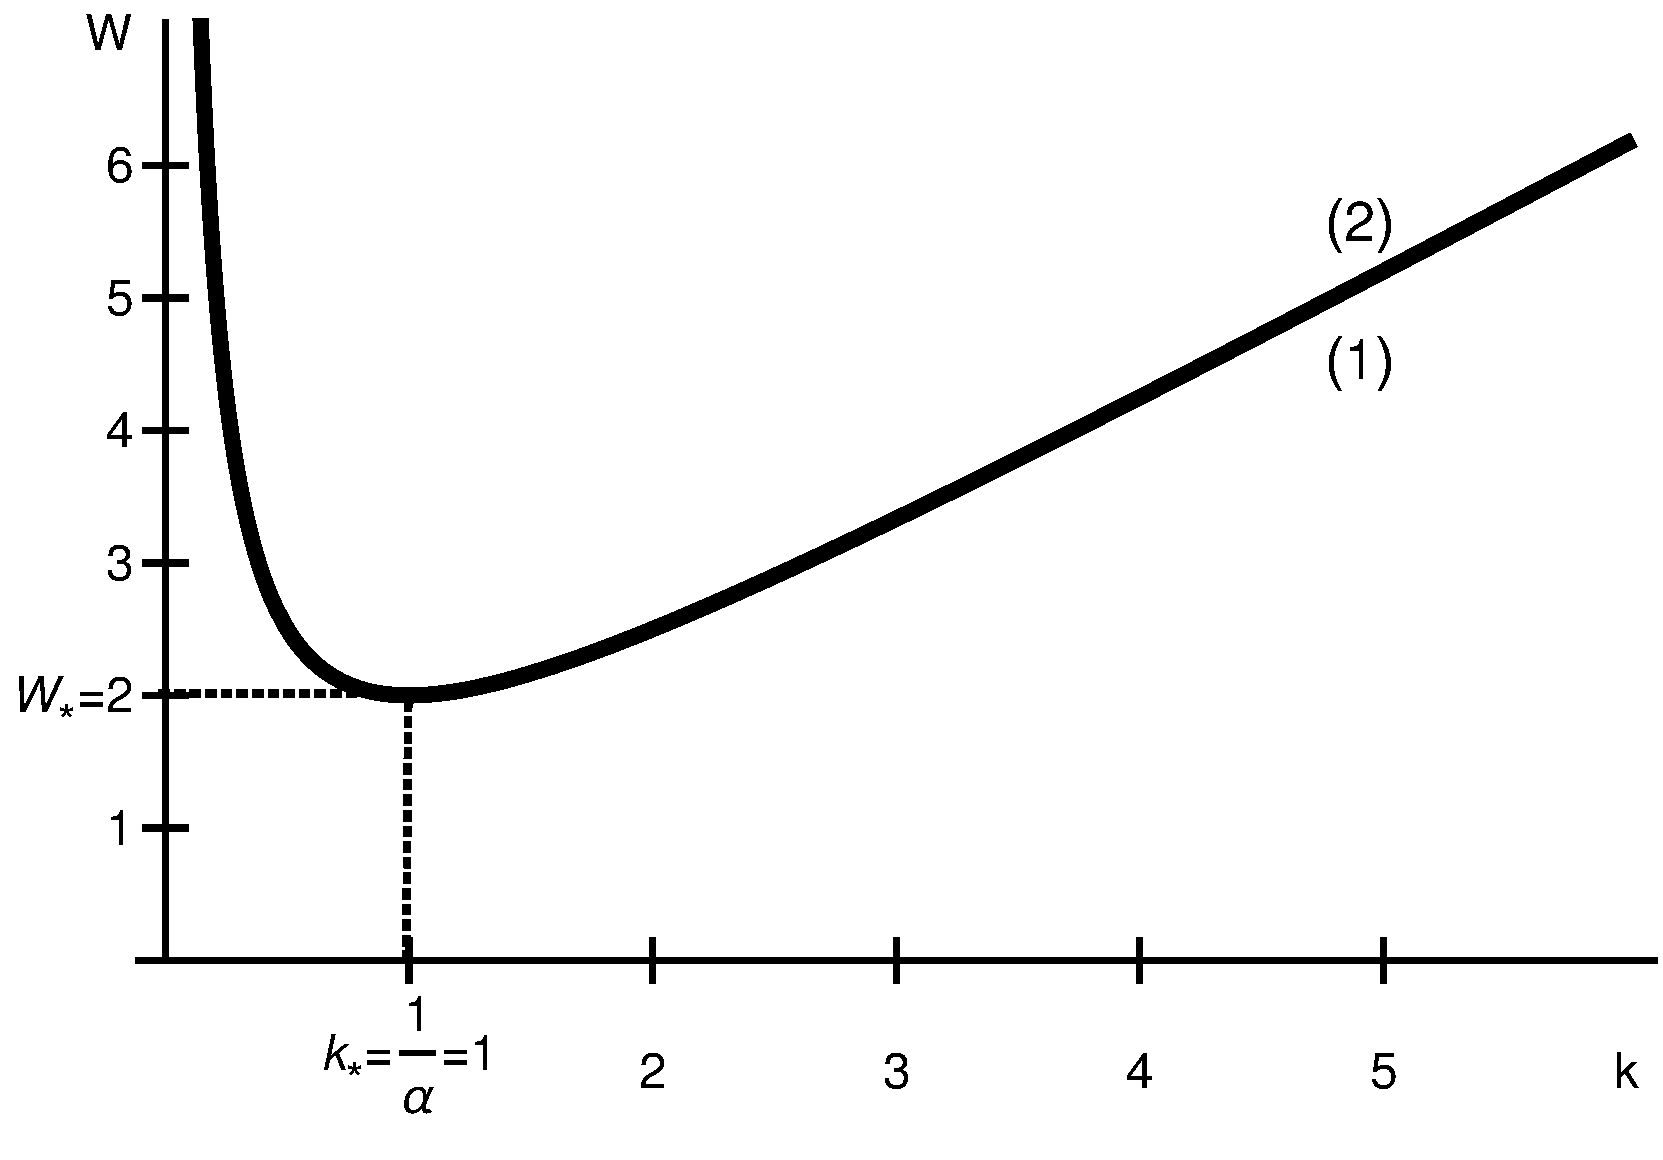
\includegraphics[scale=0.5]{T_F_Neutral}
\caption{Кривая нейтральной устойчивости неустойчивости Тонкса--Френкеля}\label{fig:NeutralW}
\end{figure}
	Область под кривой (обозначена цифрой 1) соответствует ситуации, когда капиллярные силы на вершинах волн преобладают над электрическими и возмущение свободной поверхности жидкости представляет из себя бегущую волну. Область над кривой нейтральной устойчивости (обозначена цифрой 2) определяет ситуацию, в которой электрические силы преобладают. Это соответствует апериодическому движению с развитием неустойчивости Тонкса--Френкеля и прекращением дрейфа. Для настоящей задачи интерес представляет только область устойчивого движения. Из рисунка~\ref{fig:NeutralW} видно, что существует некоторое волновое число  $ k_{cr} $, наиболее восприимчивое к поверхностному электрическому заряду. Величину  $ k_{cr} $  можно определить из условия: 
\begin{equation*}
\partial_{\alpha k}W_{cr}=0.
\end{equation*}
	 
В безразмерных переменных $ \rho=g=\gamma=1 $  волновое число примет значение  $ k_{cr}=1/\alpha=1 $. Критическое значение параметра Тонкса--Френкеля при этом  $ W_{cr}=2 $. В дальнейшем мы будем анализировать динамику движения при распространении вдоль поверхности волны с волновым числом $ k_{cr} $, поскольку именно эта волна наиболее восприимчива к неустойчивости Тонкса--Френкеля.


Интересно посмотреть, как при этом будут двигаться индивидуальные жидкие частицы. Выражения для описания траекторий движения получим, используя предложенную выше методику. Для этого необходимо записать скорость в описании Лагранжа перейдя при этом в систему координат, дрейфующую со скоростью дрейфа. С точностью до обозначений это выражение совпадет с лагранжевой скоростью, полученной при описании методики~\eqref{ul1Mod}~---~\eqref{vl1Mod}. Отличие заключается в круговой частоте, определяемой уравнением~\eqref{DUTF} и зависящей от поверхностной плотности электрического заряда. Отметим, что в предельном случае  $ W \rightarrow 0 $ осуществляется переход к классической модели Стокса. Выражения для траекторий движения индивидуальных частиц жидкости аналогичны выражениям \eqref{X}~--- \eqref{Z} с такими же оговорками. 

Электрический заряд уменьшает круговую частоту волнового движения и соответствующим образом влияет на период движения индивидуальных частиц жидкости по круговым траекториям. Таким образом, вид траекторий при значении электрического заряда меньше критического, при котором начинает развиваться неустойчивость Тонкса--Френкеля, остается таким же как и без заряда. Циклическое движение жидких частиц при этом замедляется и при достижении электрическим зарядом критического значения прекращается полностью, что соответствует переходу к апериодическому движению поверхности жидкости.
 
 
 \subsection{Заключение}
 
В присутствии поверхностного электрического заряда возмущение свободной поверхности жидкости может принять апериодический характер при превышении поверхностной плотности электрического заряда критического значения, определяемого зависимостью~\eqref{WCrit}. Существует волновое число наиболее восприимчивое к зарядовой неустойчивости. При докритических значениях поверхностной плотности электрического заряда его влияние на скорость дрейфа нелинейно.

 \section{Совокупное действие поверхностного электрического заряда и тангенциального разрыва скоростей на скорость дрейфа, связанного с распространением волнового пакета Стокса по границе раздела жидких сред}

В качестве последнего примера использования разработанной методики кажется логичным рассмотреть задачу, в которой рассматривается совокупное влияние всех рассмотренных факторов. А именно задача по расчету дрейфа и характера движения индивидуальных жидких частиц, связанного с распространением волнового пакета Стокса по границе раздела двух сред, испытывающих тангенциальный разрыв скоростей, в присутствии поверхностного электрического заряда.

Математическая формулировка задачи в этом случае будет объединять выражения ~\eqref{Euler}~---~\eqref{BeskUsl} и~\eqref{MathFormTFEul}~---~\eqref{MathFormTFBesk} и записывается следующим образом:


Задача решается аналогично предыдущим  методом разложения по малому безразмерному параметру $ \varepsilon=\zeta k $  с точностью до лидирующих слагаемых для каждого типа движения.
	  	
В нулевом порядке малости выражение для электрического потенциала записывается в точности также, как и в задаче предыдущего пункта~\ref{sec:TF}. Далее, производя снос граничных условий на уровень равновесной поверхности $ z=0 $  по известной процедуре и разбивая задачу по порядкам малости можно записать математическую формулировку задачи первого и второго порядков малости по амплитуде волнового возмущения. Задача в линейном приближении по малому параметру запишется следующим образом:

Задача второго порядка малости по амплитуде волны выглядит:

 

Решение задачи первого порядка малости  находится стандартными методами и в виде суперпозиции двух синусоидальных волн выглядит:
\begin{gather}
\xi_{1}=\zeta \cos \left( \omega_{+} t - k_{+}x \right)+\zeta \cos \left( \omega_{-} t - k_{-}x \right); \label{Xi1TFKHWP}\\
\begin{gathered}
\varphi_{1}=-\zeta \exp \left( k_{+} z \right) \dfrac{\omega_{+}}{k_{+}}\sin \left( \omega_{+} t - k_{+}x \right)-\\
-\zeta \exp \left( k_{-} z \right) \dfrac{\omega_{-}}{k_{-}}\sin \left( \omega_{-} t - k_{-}x \right); \label{phi1TFKHWP}
\end{gathered}
\\ 
\begin{gathered}
\varphi'_{1}=-\zeta \exp \left( -k_{+} z \right) \dfrac{k_{+}U_{0}-\omega_{+}}{k_{+}}\sin \left( \omega_{+} t - k_{+}x \right)-\\
-\zeta \exp \left( -k_{-} z \right) \dfrac{k_{-}U_{0}-\omega_{-}}{k_{-}}\sin \left( \omega_{-} t - k_{-}x \right); \label{phi'1TFKHWP}
\end{gathered}\\ 
\begin{gathered}
\Phi_{1}=E_{0}\zeta \cos \left( \omega_{+} t - k_{+}x \right) \exp \left( -k_{+} z \right) +\\
+E_{0}\zeta \cos \left( \omega_{-} t - k_{-}x \right) \exp \left( -k_{-} z \right).
\label{Phi1TFKHWP} 
\end{gathered}
\end{gather}
	  	
Дисперсионное уравнение определяется соотношением:
\begin{equation}
\omega = \dfrac{k \rho' U_{0}\pm \sqrt{k g \left(\rho^{2} - \rho'^{2} \right) -k^{2} \rho \rho' U_{0}^{2} + k \left( \rho + \rho' \right) \left( k \gamma - W \sqrt{\rho g \gamma} \right)}}{\rho + \rho'}
\label{DUTFKHWP}
\end{equation}
	  	
Можно заметить, что в предельном случае  $ W \rightarrow 0 $ незаряженной поверхности выражения~\eqref{Xi1TFKHWP}~---~\eqref{DUTFKHWP}  сводятся к выражениям~\eqref{ReshPackKH1Xi}~---~\eqref{ReshPackKH1Phi'} и~\eqref{DispUrKH}, полученным ранее. Также в случае перехода к одной заряженной жидкости  $ U_{0}\rightarrow 0 $, $ \rho' \rightarrow 0 $  решение задачи~\eqref{Xi1TFKHWP}~---~\eqref{DUTFKHWP}   преобразуется к виду~\eqref{xi1TF}~---~\eqref{Phi1TF},~\eqref{DUTF}. На рисунке~\ref{fig:KHWNeutralU} изображено семейство кривых нейтральной устойчивости в плоскости параметров $ \left( U_{0}, k \right) $  в безразмерных переменных  $ \rho=g=\gamma=1 $ для разных значений параметра Тонкса--Френкеля. Кривой~(1) соотвествует значение параметра Тонкса--Френкеля $ W=0 $, кривой (2)~--- $ W=1 $, кривой (3)~--- $ W=2 $, кривой (4)~--- $ W=3 $.
\begin{figure}[ht]
\centering
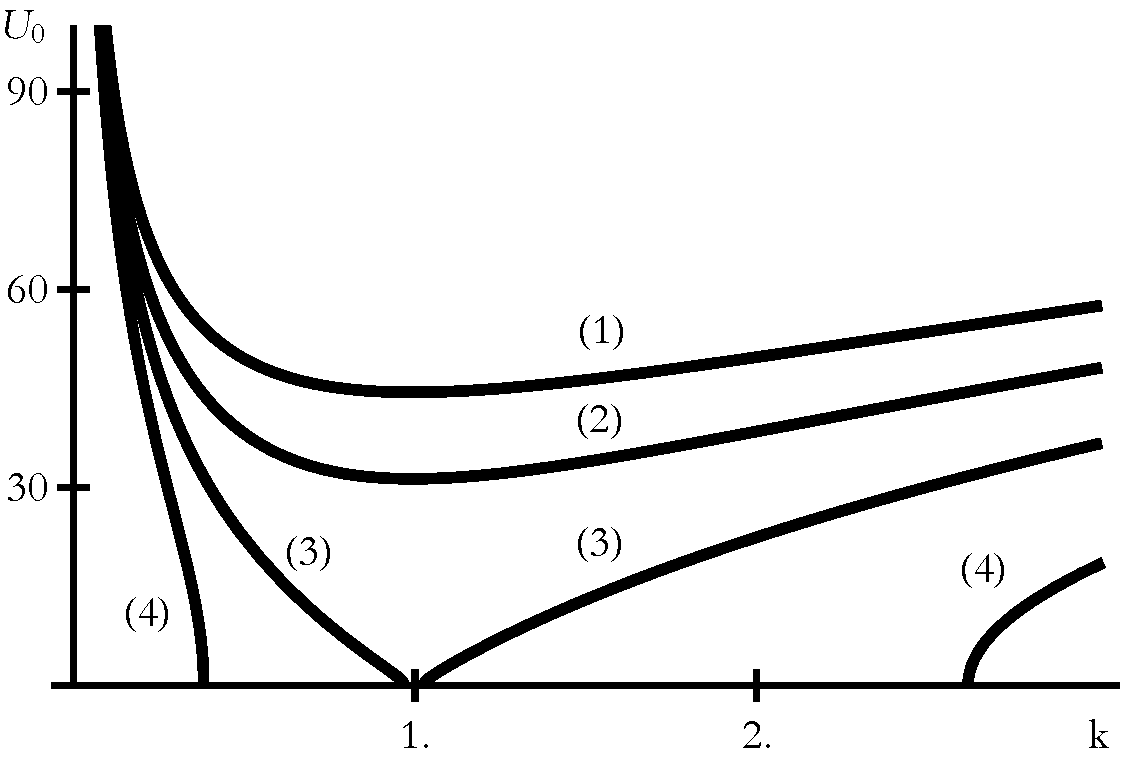
\includegraphics[scale=0.7]{Fig2a}
\caption{Кривая нейтральной устойчивости в области параметров $ \left( U_{0}, k \right) $ для разных значений параметра Тонкса--Френкеля}\label{fig:KHWNeutralU}
\end{figure}
Из графиков видно, что в присутствии поверхностного электрического заряда неустойчивость развивается при меньших значениях тангенциального разрыва скоростей. Аналогично можно построить семейство кривых нейтральной устойчивости в области параметров  $ \left( W, k \right) $ для разных значений скорости  $ U_{0} $ (рисунок~\ref{fig:KHWNeutralW}). Кривой~(1) соотвествует значение тангенциального разрыва скоростей $ U_{0}=0 $, кривой (2)~--- $ U_{0}=30 $, кривой (3)~--- $ U_{0}=44.7 $, кривой (4)~--- $ U_{0}=50 $.
\begin{figure}[ht]
\centering
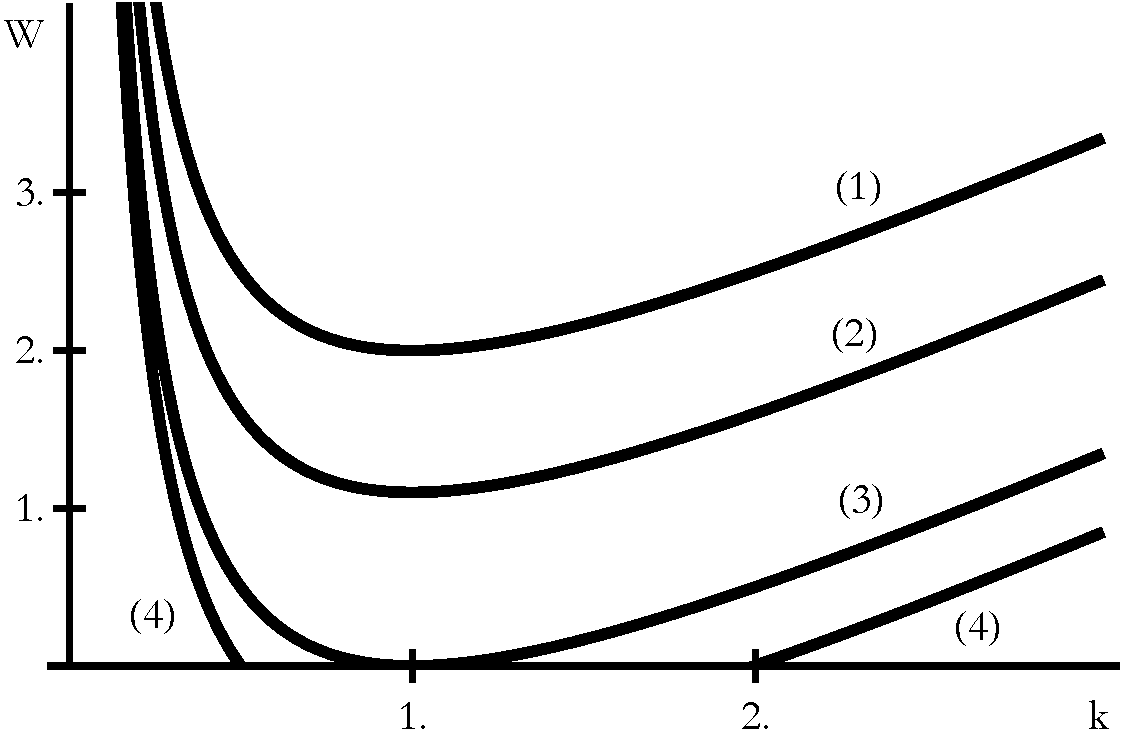
\includegraphics[scale=0.7]{Fig2b}
\caption{Кривая нейтральной устойчивости в области параметров $ \left( W, k \right) $ для разных значений тангенциального разрыва скоростей}\label{fig:KHWNeutralW}
\end{figure}
Относительное движение жидких сред снижает величину поверхностного электрического заряда, необходимого для развития неустойчивости. Таким образом дестабилизирующие факторы усиливают действие друг друга. Также можно заметить, что существует волновое число, наиболее восприимчивое к совместному действию этих дестабилизирующих факторов. В безразмерных переменных оно принимает значение  $ k_{cr}=1 $.

По аналогии с предыдущими пунктами подставим решение  в правые части граничных условий  задачи второго порядка малости и запишем их в явном виде:
\begin{gather}
\partial_{t}\xi_{2}-\partial_{z}\varphi_{2}=-2\zeta^{2}\Delta k \omega \sin \left( 2 \Delta \omega t - 2 \Delta k x \right) + \Pi \left( t \right) + O \left( \Delta k^{2} \right); \label{RPTFKHWP1}\\
\begin{gathered}
\partial_{t}\xi_{2}+U_{0} \partial_{x}\xi_{2}-\partial_{z}\varphi'_{2}=-2\zeta^{2} \Delta k \left( k U_{0} - \omega \right)\times \\
\times \sin \left( 2 \Delta \omega t - 2 \Delta k x \right) + \Pi \left( t \right) + O \left( \Delta k^{2} \right);\label{RPTFKHWP2}
\end{gathered}
\\
\Phi_{2}-E_{0}\xi_{2}=2k \zeta^{2} \sqrt{\pi W \sqrt{\rho g \gamma}} \cos \left( 2 \Delta \omega t - 2 \Delta k x \right) + \Pi \left( t \right) + O \left( \Delta k^{2} \right); \label{RPTFKHWP3}\\
\begin{gathered}
g \xi_{2} \left( \rho' - \rho \right) - \rho \partial_{t} \varphi_{2} + \rho' \partial_{t} \varphi'_{2} +\rho' U_{0} \partial_{x}\varphi'_{2} - \dfrac{E_{0}}{4 \pi}\partial_{z}\Phi_{2}+\gamma \partial_{xx}\xi_{2}=\\
=-\zeta^{2}k \left( 1+k \right) W \sqrt{\rho g \gamma} \left( \cos \left( 2 \Delta \omega t - 2 \Delta k x \right) +1\right) + \Pi \left( t \right) + O \left( \Delta k^{2} \right).
\label{RPTFKHWP4}
\end{gathered}
\end{gather}	  	
	  	
В выражениях ~\eqref{RPTFKHWP1}~---~\eqref{RPTFKHWP4}  по аналогии с предыдущими задачами символ $  \Pi \left( t \right) $  означает быстро меняющиеся со временем слагаемые. Стоит также отметить, что в правых частях оставлены только линейные слагаемые по  $ \Delta k $.
Выделяя медленно меняющиеся со временем слагаемые и решая «усеченную» задачу второго порядка малости найдем дрейфовые компоненты решения задачи второго порядка малости:
\begin{equation}
u_{d}=-2\zeta^{2} \Delta k \omega \exp \left( 2 z \Delta k \right) \cos \left( 2 \Delta \omega t - 2 \Delta k x \right)
\label{udTFKHWP} 
\end{equation}
\begin{equation}
u'_{d}=2\zeta^{2} \Delta k \left( k U_{0}-\omega\right) \exp \left( 2 z \Delta k \right) \cos \left( 2 \Delta \omega t - 2 \Delta k x \right)
\label{ud'TFKHWP} 
\end{equation}	  	
	  	
Выражения ~\eqref{udTFKHWP}~---~\eqref{ud'TFKHWP} получены с точностью до линейных слагаемых по $ \Delta k $  и формально совпадают с выражениями ~\eqref{udPacketKH}~---~\eqref{ud'PacketKH}. Отличие заключается в частоте волнового движения  $ \omega $, в нее входит поверхностный электрический заряд~\eqref{DUTFKHWP}.

Используя формулу перехода  и методику, описанную в предыдущей главе легко найти выражения для скорости дрейфа Стокса в нижней   и верхней   жидкости. Они также формально совпадают с выражениями ~\eqref{UdriftPack} с точностью до круговой частоты волнового движения $ \omega $  и частоты, измененной в соответствии с эффектом Доплера $ \Omega $:
	  		  	
С учетом смещения со скоростью дрейфа можно уточнить лагранжевые компоненты скорости индивидуальных жидких частиц и получить выражения с точностью до лидирующих слагаемых, аналогичных~\eqref{ULPackKH}~---~\eqref{UL'PackKH}.
	  	
Выражения для траекторий движения индивидуальных жидких частиц в параметрическом виде можно получить путем численного интегрирования скоростей ~\eqref{ULPackKH} для нижней жидкости и скоростей~\eqref{UL'PackKH}  для верхней, подставляя вместо частоты волнового движения $ \omega $ корректное значение~\eqref{DUTFKHWP}. Видно, что движение индивидуальных жидких частиц носит циклический характер, который в верхней жидкости не сменяется поступательным ни при каких значениях тангенциального разрыва скоростей из-за существования быстрых и медленных циклических движений. При этом частота круговых вращений жидкой частицы меньше чем частота волновой моды, вызвавшей это циклическое движение, причем чем больше скорость дрейфового движения, тем больше эта разница.

 
\section{Заключение}
 
 Разработанная методика позволяет рассчитать скорость дрейфового движения в случае сложных движений. Как показывает анализ, основные закономерности решений остаются такими же, как и в простейшем случае, но на скорость дрейфа влияют факторы,связанные с модуляцией движений и факторы, влияющие на частоту простейших волновых мод, возмущающих свободную поверхность.
 
 В качестве примеров рассмотрено влияние тангенциального разрыва скоростей, поверхностного электрического заряда, возмущение границы раздела волновым пакетом Стокса. Показано, что поверхностный электрический заряд и тангенциальный разрыв скоростей на границе раздела усиливают дестабилизирующие свойства друг друга. На начальных этапах развития неустойчивости Кельвина--Гельмгольца возникают дрейфовые течения, инициированные распространением волнового пакета по границе раздела. Дрейфовые течения направлены таким образом, чтобы уменьшить тангенциальный разрыв скоростей, вызвавший развитие неустойчивости. Однако величина дрейфовых течений оказывается примерно в два раза меньшей, чем в случае, когда дрейф инициирован простейшей синусоидальной волной. 